\part{Forced-Oscillations}
\lecture{Forced Oscillations}{Forced-Oscillations}
\section{Forced Oscillations}

\title{Ordinary Differential Equations}
\subtitle{Math 232 - Week 9, Day 2}
\date{26 October 2011}

\begin{frame}
  \titlepage
\end{frame}

\begin{frame}
  \frametitle{Outline}
  \tableofcontents[pausesection,hideothersubsections]
\end{frame}


\subsection{Forced Oscillations}


\begin{frame}
  \frametitle{Forced Oscillations}

  Section 4.1 - Redux: The governing equation for a mass/spring system
  is
  \begin{eqnarray*}
    mx'' + bx'+kx & = & f(t).
  \end{eqnarray*}

  The constants $m$, $b$, and $k$ are all non-negative.

  The function $f(t)$ is called the \textit{forcing function}.

  This is a conceptual model for many physical systems.

\end{frame}


\begin{frame}
  \frametitle{Special Case}

  Periodic forcing:
  \begin{eqnarray*}
    f(t) & = & F_0 \cos(\omega t), \\
    x(0) & = & 0, \\
    x'(0) & = & 0.
  \end{eqnarray*}

  Suppose that there is no friction, $b=0$,
  \begin{eqnarray*}
    m x'' + kx & = & F_0 \cos(\omega t).
  \end{eqnarray*}

\end{frame}


\begin{frame}
  \frametitle{Homogeneous and Particular Solution}

  \begin{eqnarray*}
    x_h & = & C_1 \cos\lp\sqrt{\frac{k}{m}}t\rp + C_2 \sin\lp\sqrt{\frac{k}{m}}t\rp.
  \end{eqnarray*}

  Assume that $\omega \neq \sqrt{\frac{k}{m}}$, then the particular
  solution is
  \begin{eqnarray*}
    x_p & = & \frac{F_0}{m\lp\frac{k}{m}-\omega^2\rp} \cos(\omega t).
  \end{eqnarray*}

\end{frame}


\begin{frame}
  \frametitle{Solve for the Constants}

  \begin{eqnarray*}
    x & = & C_1 \cos\lp\sqrt{\frac{k}{m}}t\rp + C_2 \sin\lp\sqrt{\frac{k}{m}}t\rp+ 
           \frac{F_0}{m\lp\frac{k}{m}-\omega^2\rp} \cos(\omega t).
  \end{eqnarray*}

  The initial conditions yield
  \begin{eqnarray*}
    x(0) & = & C_1 + \frac{F_0}{m\lp\frac{k}{m}-\omega^2\rp} \\
    \Rightarrow C_1 & = & \frac{-F_0}{m\lp\frac{k}{m}-\omega^2\rp}
  \end{eqnarray*}

\end{frame}


\begin{frame}
  \frametitle{Satisfy the Velocity}

  \begin{eqnarray*}
    x' & = & - C_1 \sqrt{\frac{k}{m}} \sin\lp\sqrt{\frac{k}{m}}t\rp + C_2 \sqrt{\frac{k}{m}} \cos\lp\sqrt{\frac{k}{m}}t\rp \\ 
    & & - \frac{\omega F_0}{m\lp\frac{k}{m}-\omega^2\rp} \sin(\omega t), \\
    \Rightarrow C_2 & = & 0.
  \end{eqnarray*}

  The solution is 
  \begin{eqnarray*}
    x & = & \frac{-F_0}{m\lp\frac{k}{m}-\omega^2\rp} \cos\lp\sqrt{\frac{k}{m}}t\rp 
    + \frac{F_0}{m\lp\frac{k}{m}-\omega^2\rp} \cos(\omega t).
  \end{eqnarray*}


\end{frame}


\begin{frame}
  \frametitle{Obvious Trigonometric Identity}

  \begin{eqnarray*}
    \cos(u) - \cos(v) & = & -2 \sin\lp\frac{u-v}{2}\rp \sin\lp\frac{u+v}{2}\rp.
  \end{eqnarray*}

  Our solution can be written in the form
  \begin{eqnarray*}
    x(t) & = & \frac{-F_0}{m\lp\frac{k}{m}-\omega^2\rp} \sin\lp\lp\omega-\sqrt{\frac{k}{m}}\rp t\rp
                                                        \sin\lp\lp\omega+\sqrt{\frac{k}{m}}\rp t\rp
  \end{eqnarray*}

  Plots of the equations are given on pages 262-267 in your book.

\end{frame}

\subsection{Example}

\begin{frame}                   
  \frametitle{The problem}      
                                
  A two kilogram mass is attached to a spring with constant ten N/m on
  a horizontal table. The mass is driven with a periodic force of
  \begin{eqnarray*}
    f(t) & = & 3 \cos(2t).
  \end{eqnarray*}
  the system is started from rest at the equilibrium point.

  Governing equation:
  \begin{eqnarray*}
    2 x'' + 10 x & = & 3 \cos(2t)
  \end{eqnarray*}

\end{frame}


\begin{frame}
  \frametitle{Plots}

  \only<1>{\centerline{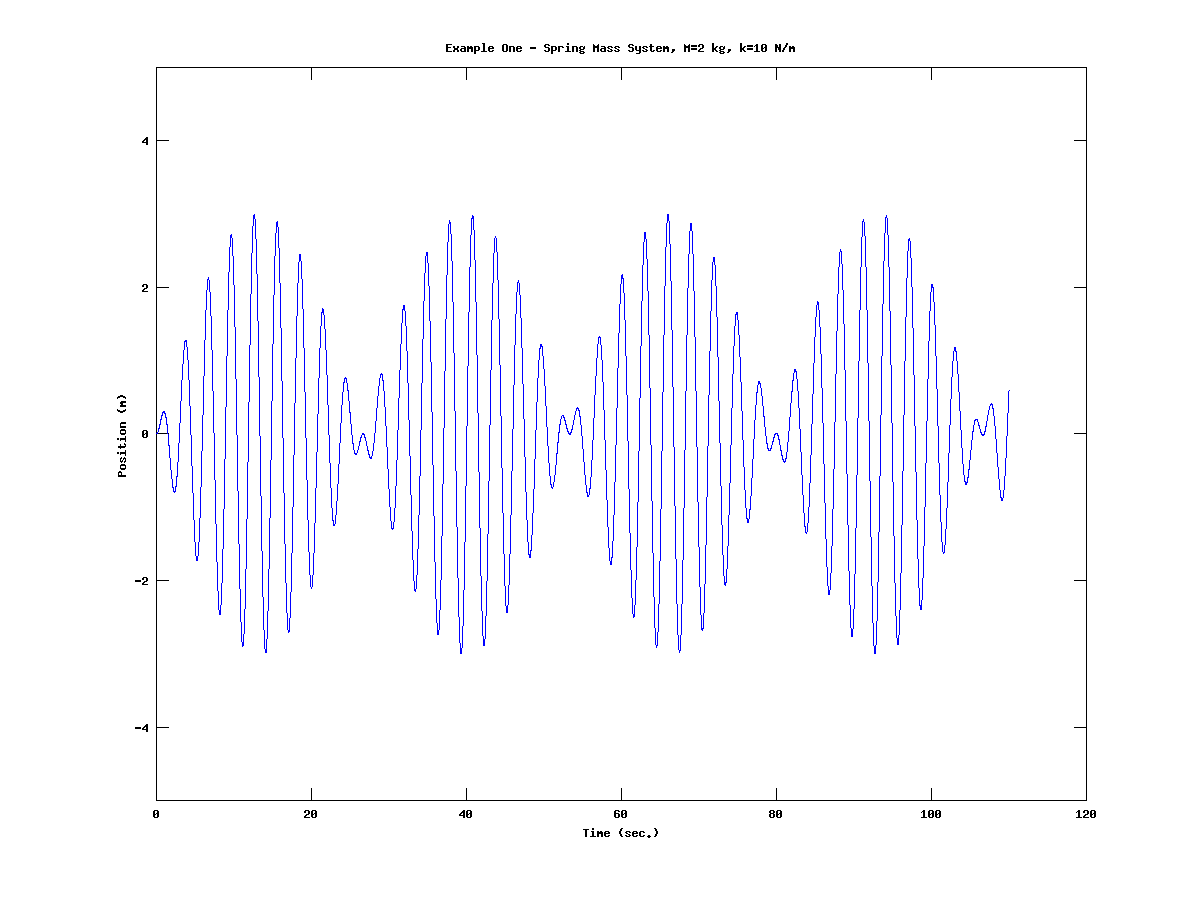
\includegraphics[width=11cm]{beats}}}
  \only<2>{\centerline{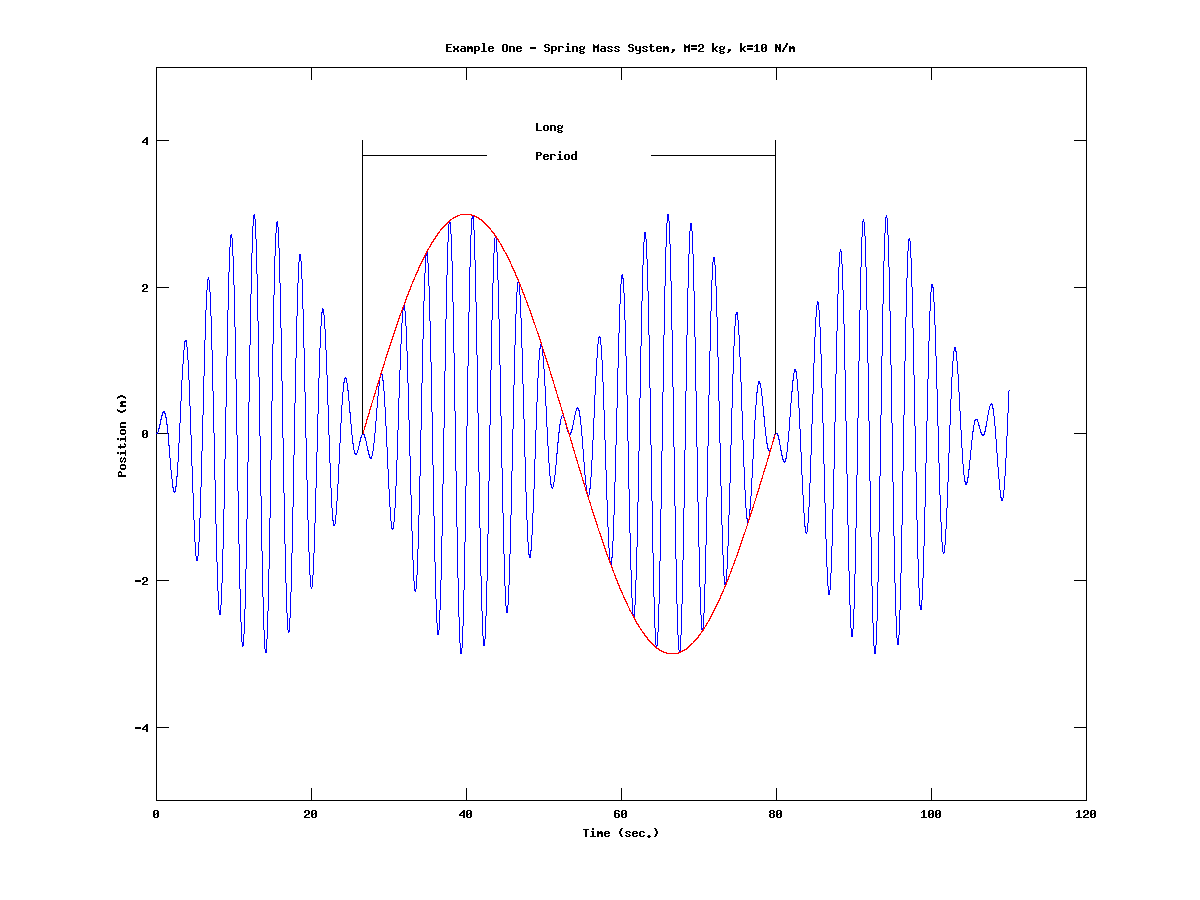
\includegraphics[width=11cm]{beatsLong}}}
  \only<3>{\centerline{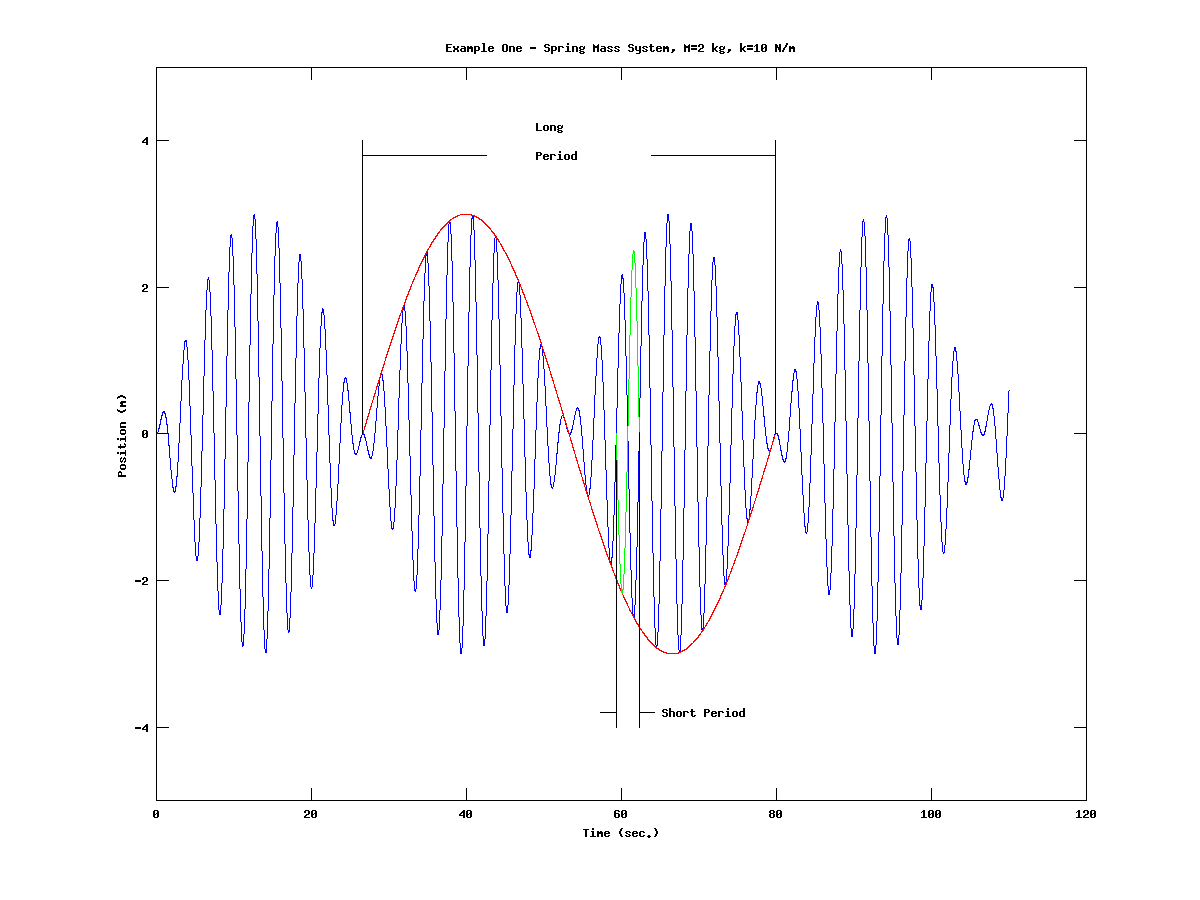
\includegraphics[width=11cm]{beatsShort}}}


\end{frame}




% LocalWords:  Clarkson pausesection hideothersubsections
